% ─────────────────────────────────────────────────────────────────────────
% Informe Taller 1 — INF3820 Procesamiento de Lenguaje Natural
% Word Embeddings (Word2Vec) y Modelado de Tópicos
% Estilo de la casa (Magíster en IA, PUC Chile)
% Compilar: pdflatex -> pdflatex   (o: tectonic informe_taller1_w2v.tex)
% ─────────────────────────────────────────────────────────────────────────
\documentclass[12pt, a4paper]{article}

\usepackage[utf8]{inputenc}
\usepackage[T1]{fontenc}
\usepackage[spanish,es-tabla]{babel}
\usepackage{geometry}
\usepackage{setspace}
\usepackage{parskip}
\usepackage{hyperref}
\usepackage{enumitem}
\usepackage{titlesec}
\usepackage{fancyhdr}
\usepackage{xcolor}
\usepackage[authoryear,round]{natbib}
\usepackage{graphicx}
\usepackage{tikz}
\usepackage{booktabs}
\usepackage{array}
\usepackage{caption}
\usepackage{float}
\usepackage{amsmath}
\usepackage{amssymb}

\geometry{margin=2.5cm}
\onehalfspacing
\graphicspath{{figures/}{./}}

% ── Colores UC ──
\definecolor{accent}{RGB}{0, 90, 130}
\definecolor{ucblue}{RGB}{0, 75, 135}
\definecolor{ucgold}{RGB}{198, 166, 80}

% ── Formato de secciones ──
\titleformat{\section}{\large\bfseries\color{accent}}{\thesection.\ }{0.3em}{}[\vspace{-0.5em}\color{accent}\rule{\textwidth}{0.4pt}]
\titleformat{\subsection}{\normalsize\bfseries\color{accent!80!black}}{\thesubsection\ }{0.3em}{}

% ── Encabezado ──
\pagestyle{fancy}
\fancyhf{}
\fancyhead[L]{\small\textit{Taller 1: Word Embeddings y Modelado de Tópicos}}
\fancyhead[R]{\small\textit{INF3820}}
\fancyfoot[C]{\thepage}
\renewcommand{\headrulewidth}{0.4pt}

\captionsetup{font=small,labelfont=bf}
\newcommand{\code}[1]{\texttt{#1}}

\hypersetup{
    colorlinks=true,
    linkcolor=accent,
    urlcolor=accent!70!black,
    citecolor=accent,
    pdftitle={Taller 1 - INF3820: Word Embeddings (Word2Vec) y Modelado de Topicos},
    pdfauthor={Julynho Toledo Rios, Armando Arredondo Valle, Thyare Parra Santander},
    pdfsubject={Procesamiento de Lenguaje Natural},
    pdfkeywords={Word2Vec, CBOW, Skip-gram, PCA, K-Means, document embeddings}
}

% ══════════════════════════════════════════════════════════════════════
\begin{document}

% ── Portada ──
\begin{titlepage}
    \begin{tikzpicture}[remember picture, overlay]
        \fill[ucblue] (current page.north west) rectangle ([yshift=-4cm]current page.north east);
        \fill[ucgold] ([yshift=-4cm]current page.north west) rectangle ([yshift=-4.15cm]current page.north east);
        \fill[ucblue] (current page.south west) rectangle ([yshift=2cm]current page.south east);
        \fill[ucgold] ([yshift=2cm]current page.south west) rectangle ([yshift=2.15cm]current page.south east);
    \end{tikzpicture}

    \centering
    \singlespacing
    \vspace*{0.8cm}

    
\includegraphics[width=4.8cm]{Logo.png}

    \vspace{1.1cm}

    {\color{ucblue}\rule{0.6\textwidth}{0.8pt}}

    \vspace{0.7cm}

    {\LARGE\bfseries\color{ucblue} Taller 1\\[0.35em]
    Word Embeddings (Word2Vec)\\[0.25em] y Modelado de Tópicos}

    \vspace{0.9cm}

    {\large\color{black} CBOW frente a Skip-gram, analogías vectoriales,\\[0.3em]
    proyección PCA y agrupamiento de documentos\\[0.3em]
    sobre un corpus de economía chilena}

    \vspace{0.7cm}

    {\color{ucblue}\rule{0.6\textwidth}{0.8pt}}

    \vspace{1.0cm}

    {\large\bfseries Integrantes del grupo}

    \vspace{0.4cm}

    {\normalsize Julynho Merlin Toledo Rios\\[0.2em]
    Armando Arredondo Valle\\[0.2em]
    Thyare Graciela Parra Santander}

    \vspace{0.9cm}

    {\normalsize Maestría en Inteligencia Artificial\\[0.25em]
    INF3820 -- Procesamiento de Lenguaje Natural\\[0.25em]
    Prof. Rodrigo Andres Sandoval Urrich\\[0.25em]
    Pontificia Universidad Católica de Chile}

    \vfill

    {\normalsize Agosto de 2026}

    \vspace{1.2cm}
\end{titlepage}

% ═════════════════════════════════════════════════════════════════
\section{Introducción}

Los \textit{word embeddings} son representaciones densas de palabras en un espacio vectorial
continuo, aprendidas a partir de la coocurrencia de términos en un corpus. Word2Vec
\citep{mikolov2013efficient, mikolov2013distributed} popularizó dos arquitecturas para construirlas:
CBOW (\textit{Continuous Bag of Words}), que predice una palabra objetivo a partir de su contexto, y
Skip-gram, que invierte el problema y predice el contexto a partir de la palabra objetivo. La
promesa de ambas es que la geometría del espacio resultante codifica relaciones semánticas, de modo
que la proximidad entre vectores y las operaciones aritméticas sobre ellos permiten recuperar
analogías y agrupar textos por tema.

Este informe reporta los resultados del Taller 1 del curso, cuyo objetivo es cuádruple: comparar
empíricamente CBOW y Skip-gram, operar algebraicamente con los embeddings para identificar
relaciones semánticas, proyectar el espacio de alta dimensión a dos dimensiones mediante PCA, y
construir un agrupador de tópicos a partir de \textit{document embeddings} obtenidos por promedio de
vectores. El material de trabajo es un corpus sintético de doce oraciones sobre economía e industria
en Chile (minería, energía, finanzas y regulación ambiental), lo que introduce una restricción que
resulta ser el hilo conductor de todo el análisis: con tan poca evidencia, buena parte de lo que se
observa se explica más por el tamaño del corpus que por las propiedades teóricas de cada
arquitectura.

El documento se organiza como sigue. La Sección 2 describe el corpus y la configuración
experimental. Las secciones 3 a 6 presentan los resultados de los cuatro ejercicios: comparación de
arquitecturas, aritmética de analogías, proyección PCA y modelado de tópicos con K-Means. La
Sección 7 recoge la discusión final sobre las limitaciones del promedio de vectores, la comparación
frente a métodos clásicos y el aporte de los embeddings contextuales. La Sección 8 cierra con las
conclusiones.

% ═════════════════════════════════════════════════════════════════
\section{Corpus y configuración experimental}

\subsection{Descripción del corpus}

El corpus está compuesto por doce oraciones en español, construidas para cubrir cuatro ejes
temáticos de la economía chilena: minería, energía, finanzas y regulación ambiental. La Tabla
\ref{tab:corpus} lista los documentos junto con el eje temático que se les puede asignar por
inspección, referencia que se usará más adelante para evaluar la calidad del agrupamiento
automático.

\begin{table}[H]
\centering
\caption{Corpus de trabajo: doce documentos y su tema asignado por inspección.}
\label{tab:corpus}
\small
\renewcommand{\arraystretch}{1.15}
\begin{tabular}{@{}cp{9.2cm}l@{}}
\toprule
\textbf{ID} & \textbf{Documento} & \textbf{Tema} \\
\midrule
D1  & La minería de cobre en el norte de Chile requiere alta eficiencia energética & Minería/Energía \\
D2  & El litio es un mineral clave para la transición energética y las baterías & Minería/Energía \\
D3  & El banco central ajustó la tasa de interés para controlar la inflación acumulada & Finanzas \\
D4  & Las instituciones financieras evalúan el riesgo crediticio en la economía local & Finanzas \\
D5  & La energía solar y eólica lideran la matriz limpia en la región de Antofagasta & Energía \\
D6  & El precio del cobre impacta directamente los ingresos fiscales del Estado chileno & Minería/Finanzas \\
D7  & Los analistas económicos proyectan un crecimiento moderado del producto interno bruto & Finanzas \\
D8  & Proyectos de minería verde buscan reducir el consumo de agua en procesos industriales & Minería/Ambiental \\
D9  & La regulación ambiental exige evaluaciones de impacto para nuevos proyectos de energía & Ambiental \\
D10 & El sistema financiero local mantiene altos estándares de liquidez y capitalización & Finanzas \\
D11 & La producción de litio en los salares requiere innovaciones en extracción directa & Minería \\
D12 & La tasa de desempleo y la inflación influyen en las decisiones del banco central & Finanzas \\
\bottomrule
\end{tabular}
\end{table}

\subsection{Preprocesamiento y configuración de los modelos}

Cada documento se tokenizó con la utilidad \code{simple\_preprocess} de Gensim
\citep{rehurek2010software}, que normaliza a minúsculas y descarta puntuación y tokens muy cortos, y
a continuación se filtraron las palabras vacías del español provistas por NLTK. El resultado son
doce listas de tokens de contenido: por ejemplo, D1 queda reducido a
\code{[minería, cobre, norte, chile, requiere, alta, eficiencia, energética]}.

Este dato es relevante para interpretar todo lo que sigue: tras el filtrado, cada documento conserva
entre siete y nueve tokens. Es decir, el corpus completo ronda el centenar de tokens de contenido y
la mayoría de las palabras del vocabulario aparece una o dos veces.

Los modelos se entrenaron con dimensión de embedding igual a 60, ventana de contexto 3, frecuencia
mínima 1 y 200 épocas, fijando la semilla en 42. El entrenamiento se ejecutó con un solo hilo de
trabajo, condición necesaria para que la semilla garantice reproducibilidad exacta: con varios hilos
el orden de las actualizaciones asincrónicas deja de ser determinista. Se entrenaron dos modelos con
idéntica configuración salvo la arquitectura, uno CBOW y otro Skip-gram.

% ═════════════════════════════════════════════════════════════════
\section{Ejercicio 1: entrenamiento comparativo CBOW frente a Skip-gram}

\subsection{Vecinos más cercanos de \textit{cobre}}

La Tabla \ref{tab:e1} presenta las tres palabras más similares a \code{cobre} en cada arquitectura
bajo la configuración base.

\begin{table}[H]
\centering
\caption{Tres vecinos más cercanos de \code{cobre} por arquitectura (\code{window}\,=\,3, similitud coseno).}
\label{tab:e1}
\small
\renewcommand{\arraystretch}{1.2}
\begin{tabular}{@{}clc lc@{}}
\toprule
\textbf{Puesto} & \multicolumn{2}{c}{\textbf{CBOW}} & \multicolumn{2}{c}{\textbf{Skip-gram}} \\
\cmidrule(lr){2-3}\cmidrule(lr){4-5}
 & Palabra & Similitud & Palabra & Similitud \\
\midrule
1.º & solar    & 0,642 & local  & 0,928 \\
2.º & local    & 0,636 & solar  & 0,914 \\
3.º & requiere & 0,618 & matriz & 0,913 \\
\bottomrule
\end{tabular}
\end{table}

La observación central es que ambas arquitecturas devuelven prácticamente los mismos vecinos
(\code{solar} y \code{local} aparecen en las dos listas), de modo que la diferencia relevante no está
en qué palabras se recuperan sino en los puntajes. CBOW entrega similitudes entre 0,618 y 0,642,
mientras que en Skip-gram los tres primeros superan 0,913 y quedan casi empatados entre sí.

La explicación está en la forma de entrenar de cada arquitectura. Skip-gram genera un ejemplo de
entrenamiento por cada par (palabra, contexto), de manera que con 200 épocas sobre doce oraciones el
espacio termina fuertemente comprimido: casi todos los vectores apuntan en direcciones parecidas,
las similitudes se inflan y el modelo pierde capacidad de discriminar entre un vecino y otro. CBOW,
en cambio, promedia los vectores del contexto antes de predecir, lo que suaviza las actualizaciones y
deja un espacio menos saturado, en el que los puntajes todavía permiten ordenar candidatos.

Llama la atención que ninguno de los dos modelos entregue términos del dominio minero para
\code{cobre}. Revisando el corpus la razón es clara: \code{cobre} aparece solo en dos documentos (D1,
sobre eficiencia energética, y D6, sobre ingresos fiscales), y con esa evidencia el modelo no alcanza
a anclar la palabra a un campo semántico. Sus vecinos terminan siendo simplemente términos con los
que coocurre.

\subsection{Sensibilidad al tamaño de la ventana}

Para la pregunta 1.2 se repitió el entrenamiento variando \code{window} entre 3 y 10, manteniendo
constante todo lo demás. La Tabla \ref{tab:window} resume los resultados.

\begin{table}[H]
\centering
\caption{Tres vecinos más cercanos de \code{cobre} al variar el tamaño de ventana.}
\label{tab:window}
\small
\renewcommand{\arraystretch}{1.2}
\begin{tabular}{@{}c>{\raggedright\arraybackslash}p{5.4cm}>{\raggedright\arraybackslash}p{5.4cm}@{}}
\toprule
\textbf{Ventana} & \textbf{CBOW} & \textbf{Skip-gram} \\
\midrule
3  & solar (0,642), local (0,636), requiere (0,618)   & local (0,928), solar (0,914), matriz (0,913) \\
5  & local (0,748), requiere (0,737), impacta (0,728) & requiere (0,973), local (0,973), impacta (0,972) \\
7  & requiere (0,744), solar (0,727), verde (0,721)   & requiere (0,979), proyectos (0,978), matriz (0,975) \\
10 & solar (0,768), local (0,745), requiere (0,729)   & solar (0,982), local (0,982), requiere (0,980) \\
\bottomrule
\end{tabular}
\end{table}

Los vecinos de \code{cobre} no se especializan en minería al aumentar la ventana; ocurre lo
contrario. Se vuelven más genéricos y cada vez más difíciles de separar entre sí: con
\code{window}\,=\,10 en Skip-gram los tres primeros quedan entre 0,980 y 0,982, es decir, la
geometría se aplana hasta el punto en que casi cualquier palabra del corpus queda cerca de
\code{cobre}.

En teoría una ventana pequeña captura relaciones locales y sintácticas, ligadas a la posición de la
palabra en la oración, mientras que una ventana amplia captura relaciones temáticas. Aquí pesa más
una consideración práctica: como cada oración conserva entre siete y nueve tokens tras eliminar las
palabras vacías, una ventana de 10 cubre la oración completa y el contexto de cada palabra pasa a ser
todo su documento. En esas condiciones dos palabras resultan similares por el solo hecho de compartir
oración, lo que homogeneiza el espacio. De hecho, los vecinos que se repiten en todas las
configuraciones (\code{requiere}, \code{local}, \code{solar}) son palabras que coocurren con
\code{cobre} o que aparecen en varias oraciones, no términos propios de la minería. En un corpus de
este tamaño, agrandar la ventana no especializa la representación: solo diluye la señal.

% ═════════════════════════════════════════════════════════════════
\section{Ejercicio 2: álgebra vectorial y analogías semánticas}

Se evaluó la analogía \textit{cobre es a minería lo que inflación es a X} mediante la operación
$v_{\text{minería}} - v_{\text{cobre}} + v_{\text{inflación}}$, y se recuperaron las palabras más
cercanas al vector resultante en ambos modelos. La Tabla \ref{tab:analogia} presenta los cinco
primeros resultados.

\begin{table}[H]
\centering
\caption{Palabras más cercanas al vector $v_{\text{minería}} - v_{\text{cobre}} + v_{\text{inflación}}$.}
\label{tab:analogia}
\small
\renewcommand{\arraystretch}{1.2}
\begin{tabular}{@{}clclc@{}}
\toprule
\textbf{Puesto} & \multicolumn{2}{c}{\textbf{Skip-gram}} & \multicolumn{2}{c}{\textbf{CBOW}} \\
\cmidrule(lr){2-3}\cmidrule(lr){4-5}
 & Palabra & Similitud & Palabra & Similitud \\
\midrule
1.º & minería    & 0,8209 & minería    & 0,6290 \\
2.º & inflación  & 0,7978 & inflación  & 0,5077 \\
3.º & impacto    & 0,7432 & impacto    & 0,4038 \\
4.º & tasa       & 0,7218 & crediticio & 0,2989 \\
5.º & crediticio & 0,7094 & influyen   & 0,2726 \\
\bottomrule
\end{tabular}
\end{table}

\subsection{Interpretación del espacio vectorial}

Antes de interpretar conviene una precisión metodológica: como la consulta se hizo pasando el vector
resultante en bruto y no los nombres de las palabras, la función de búsqueda no excluye los términos
de entrada. Por eso \code{minería} (0,8209) e \code{inflación} (0,7978) encabezan la lista, algo
esperable dado que el vector resultante conserva buena parte de ambos. Lo informativo son las
primeras palabras nuevas: \code{impacto} (0,7432), \code{tasa} (0,7218) y \code{crediticio} (0,7094),
todas del ámbito financiero y monetario.

La relación que captura el modelo es la de un concepto con el dominio que lo gestiona. Así como
\code{cobre} es el objeto material de la \code{minería}, la \code{inflación} es la variable central
del aparato monetario, en el que la \code{tasa} es el instrumento de control y el banco central la
institución que la administra. La resta $v_{\text{minería}} - v_{\text{cobre}}$ aísla, de forma
gruesa, la dirección de ``actividad que engloba al objeto'', y al sumarla a \code{inflación} el
vector cae en la zona del espacio ocupada por los términos de política monetaria. Que esto funcione
con doce oraciones se explica porque el corpus es fuertemente temático: \code{inflación} coocurre
únicamente con \code{banco}, \code{central} y \code{tasa}.

\subsection{Estrategias para mejorar la precisión de la analogía}

La estrategia de mayor rendimiento es partir de embeddings preentrenados sobre corpus masivos:
\code{word2vec-google-news-300} para inglés o, en nuestro caso, alternativas en español como los
vectores del \textit{Spanish Billion Word Corpus} o fastText en español
\citep{bojanowski2017enriching}. Esos modelos ya observaron millones de contextos en los que
\code{cobre} aparece junto a \code{minería}, \code{yacimiento} o \code{Codelco}, de modo que la
dirección de la analogía viene aprendida de manera robusta, mientras que en nuestro corpus esa
relación depende de apenas dos coocurrencias. La vía alternativa es ampliar el corpus, por ejemplo
con miles de noticias económicas chilenas; también funciona, pero alcanzar el mismo nivel exige mucho
más esfuerzo. Entre las opciones preentrenadas, fastText tiene la ventaja adicional de operar con
subpalabras, lo que le permite generalizar incluso a términos no vistos en entrenamiento.

\subsection{Sensibilidad de la analogía a la arquitectura}

Al repetir la operación con CBOW (columnas derechas de la Tabla \ref{tab:analogia}) la dirección
semántica se conserva solo parcialmente. \code{impacto} y \code{crediticio} reaparecen, señal de que
el vector sigue apuntando a la zona financiera, pero la analogía se degrada de forma apreciable: las
similitudes caen a menos de la mitad (0,4038 frente a 0,7432 para la primera palabra nueva) y
\code{tasa}, que era el resultado más limpio en Skip-gram, desaparece del top-5, reemplazada por
\code{influyen}, semánticamente poco informativa.

La razón está en cómo distribuye los pesos cada arquitectura. CBOW promedia los vectores del contexto
antes de predecir, lo que suaviza las representaciones y hace que las palabras frecuentes dominen el
aprendizaje, mientras que las poco frecuentes reciben actualizaciones diluidas; en este corpus casi
todo el vocabulario aparece una o dos veces. Skip-gram entrena cada par palabra-contexto por separado
y deja a los términos raros con vectores mejor definidos. Como la aritmética de analogías requiere
que \code{cobre}, \code{minería} e \code{inflación} tengan direcciones nítidas, la arquitectura que
mejor representa palabras infrecuentes, es decir Skip-gram, entrega el resultado más interpretable.
Con CBOW el concepto general se conserva, pero la precisión se pierde.

% ═════════════════════════════════════════════════════════════════
\section{Ejercicio 3: reducción de dimensionalidad y visualización}

Se extrajo el vocabulario completo del modelo Skip-gram junto con sus vectores de 60 dimensiones y se
proyectó a dos dimensiones mediante PCA. La Figura \ref{fig:pca} muestra la proyección resultante con
las etiquetas de cada término.

\begin{figure}[H]
\centering
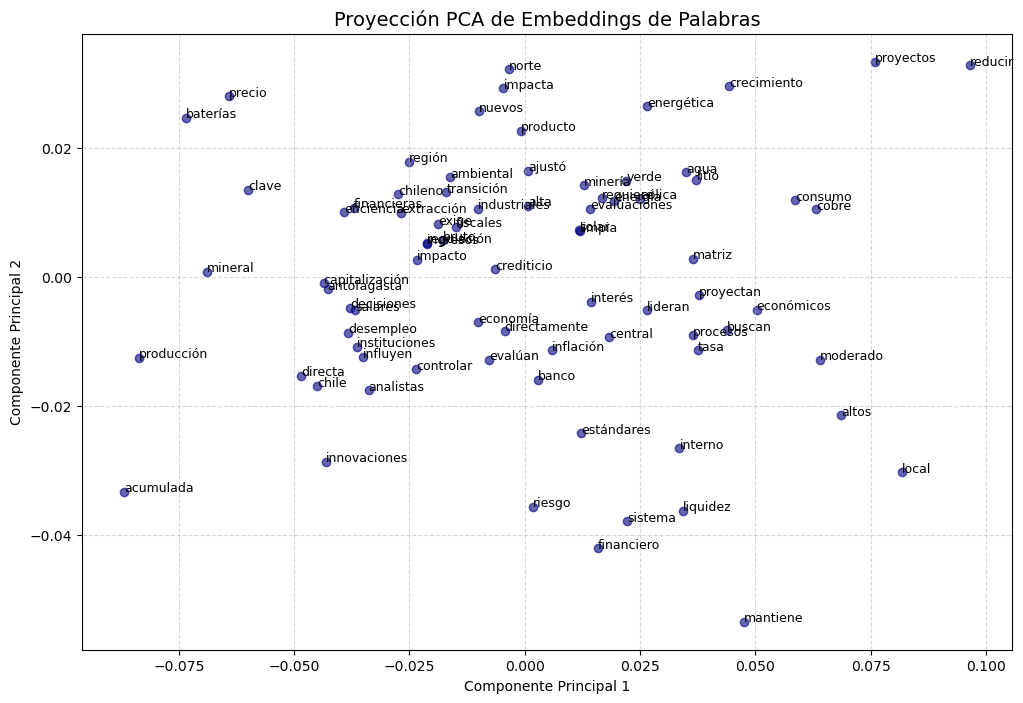
\includegraphics[width=\textwidth]{pca_embeddings.png}
\caption{Proyección PCA de los embeddings de palabras del modelo Skip-gram (60 dimensiones a 2
dimensiones). Los dos primeros componentes explican en conjunto un 24,37\,\% de la varianza.}
\label{fig:pca}
\end{figure}

\subsection{Varianza explicada y agrupaciones observadas}

Antes de buscar agrupaciones conviene cuantificar cuánta información sobrevive a la proyección: PC1
explica un 19,77\,\% de la varianza y PC2 un 4,60\,\%, para un total de 24,37\,\%. El gráfico es, por
tanto, un resumen bastante parcial del espacio original.

Aun así se distinguen agrupaciones lógicas, más como vecindades difusas que como conglomerados
nítidos. La más clara es la financiera: \code{inflación}, \code{banco}, \code{central},
\code{interés}, \code{economía}, \code{evalúan} y \code{controlar} ocupan una franja contigua en la
zona centro-inferior del plano. Hacia el centro-derecha superior se organiza una vecindad
minero-energética con \code{minería}, \code{verde}, \code{agua}, \code{litio}, \code{energía},
\code{eólica} y \code{evaluaciones}.

\subsection{Preservación de las cercanías tras la proyección}

Para evaluar objetivamente si la cercanía semántica sobrevive a la reducción se compararon, para
cuatro pares de interés, la similitud coseno en el espacio original de 60 dimensiones con la
distancia euclidiana en el plano proyectado. La Tabla \ref{tab:pca} recoge estos valores junto con la
distancia media entre todos los pares del vocabulario en 2D, que sirve como referencia.

\begin{table}[H]
\centering
\caption{Preservación de cercanías tras la proyección PCA. La distancia 2D media entre todos los
pares del vocabulario es 0,054.}
\label{tab:pca}
\small
\renewcommand{\arraystretch}{1.2}
\begin{tabular}{@{}lccl@{}}
\toprule
\textbf{Par} & \textbf{Coseno en 60D} & \textbf{Distancia en 2D} & \textbf{¿Se preserva?} \\
\midrule
banco -- central     & 0,825 & 0,017 & Sí, muy por debajo de la media \\
inflación -- tasa    & 0,872 & 0,032 & Sí, por debajo de la media \\
cobre -- minería     & 0,876 & 0,050 & No, queda en la media \\
litio -- baterías    & 0,758 & 0,111 & No, al doble de la media \\
\bottomrule
\end{tabular}
\end{table}

El resultado es desigual. El par \code{inflación}--\code{tasa}, con coseno 0,872 en 60 dimensiones,
queda a distancia 0,032 en el plano, y \code{banco}--\code{central} (0,825) a 0,017; ambos claramente
por debajo de la distancia media de 0,054, lo que indica que esas relaciones sobreviven a la
proyección. El par \code{cobre}--\code{minería}, en cambio, presenta la similitud más alta del
conjunto en 60 dimensiones (0,876) pero queda a 0,050 en 2D, prácticamente la distancia promedio; en
la Figura \ref{fig:pca} \code{cobre} aparece en el extremo derecho, lejos de \code{minería}. El caso
\code{litio}--\code{baterías} es aún más extremo, con una distancia proyectada que duplica la media.

Aquí se manifiesta la limitación estructural de PCA: al tratarse de una proyección lineal que
maximiza la varianza global, no ofrece garantía alguna de conservar las vecindades locales. La
dirección que unía \code{cobre} con \code{minería} sencillamente no quedó alineada con los dos
primeros componentes. Para estudiar vecindades locales sería más apropiado t-SNE
\citep{vandermaaten2008visualizing}, que optimiza justamente la preservación de la estructura local
en lugar de la varianza global.

% ═════════════════════════════════════════════════════════════════
\section{Ejercicio 4: modelado de tópicos con \textit{document embeddings}}

Cada documento se representó mediante \textit{mean pooling}, es decir, el promedio de los vectores
Skip-gram de las palabras presentes en el vocabulario del modelo, descartando los tokens fuera de
vocabulario. Sobre la matriz de doce representaciones resultante se aplicó K-Means con $K=3$. La
Tabla \ref{tab:clusters} presenta la asignación obtenida.

\begin{table}[H]
\centering
\caption{Asignación de documentos a tópicos mediante K-Means ($K=3$) sobre \textit{document embeddings}.}
\label{tab:clusters}
\small
\renewcommand{\arraystretch}{1.2}
\begin{tabular}{@{}clp{7.2cm}@{}}
\toprule
\textbf{Cluster} & \textbf{Documentos} & \textbf{Lectura temática} \\
\midrule
1 & D1, D4, D5, D7, D8, D9, D10 & Mezcla de minería, energía, regulación ambiental y finanzas; sin tema unificador \\
2 & D2, D6, D11                 & Commodities y su valor económico (litio y precio del cobre) \\
3 & D3, D12                     & Política monetaria (banco central, tasa, inflación) \\
\bottomrule
\end{tabular}
\end{table}

\subsection{Calidad y coherencia del agrupamiento}

La separación funcionó a medias. El cluster 3 quedó impecable: aisló exactamente los dos documentos
de política monetaria, que comparten casi todo su vocabulario (\code{banco}, \code{central},
\code{tasa}, \code{inflación}). El cluster 2 también admite lectura, con un matiz: reúne los dos
documentos sobre litio con el del precio del cobre, de modo que más que minería en sentido estricto
conforma un tópico de commodities y su valor económico.

El problema es el cluster 1, que operó como cajón de sastre. Mezcla documentos minero-energéticos con
tres claramente financieros: D4 (instituciones financieras y riesgo crediticio), D10 (sistema
financiero, liquidez y capitalización) y D7 (analistas y producto interno bruto), que por tema
deberían haber caído junto al cluster 3. Esos tres son los documentos fuera de lugar.

El \textit{mean pooling} explica en buena medida esa asignación. Al promediar todos los vectores del
documento, los términos discriminativos (\code{crediticio}, \code{liquidez}) se diluyen entre
palabras genéricas que cruzan todo el corpus (\code{local}, \code{requiere}, \code{proyectan},
\code{evalúan}), que como se vio en el Ejercicio 1 son precisamente las que el modelo dejó cerca de
todo. El promedio arrastra los \textit{document embeddings} hacia el centro común del espacio, y esos
documentos financieros terminan más próximos al centroide genérico del cluster 1 que al núcleo
monetario, que es pequeño y compacto.

\subsection{Representación global frente a local: alternativas al promedio simple}

En este taller los artículos y preposiciones se filtraron con las palabras vacías de NLTK antes de
entrenar, de modo que no contaminan directamente el promedio. El fenómeno de fondo, sin embargo,
persiste bajo la forma de lo que podría llamarse palabras vacías de dominio: términos como
\code{requiere}, \code{local} o \code{proyectos}, frecuentes en el corpus pero poco útiles para
distinguir tópicos, pesan en el promedio exactamente igual que \code{litio} o \code{crediticio}. De
no haberse eliminado las palabras vacías el efecto sería peor: al ser las más frecuentes, dominarían
el promedio y empujarían todos los documentos hacia un mismo punto del espacio, borrando las
diferencias temáticas.

Una mejora directa consiste en ponderar el promedio con TF-IDF, multiplicando cada vector por la
relevancia del término en el documento respecto del corpus. Bajo ese esquema \code{crediticio}, raro
y discriminativo, pesaría mucho más que \code{requiere}, transversal. Una variante más refinada es
SIF (\textit{Smooth Inverse Frequency}), que pondera cada palabra por $a/(a + p(w))$ y además remueve
el primer componente principal común a todos los documentos \citep{arora2017simple}. Si se quiere
abandonar el promedio por completo, Doc2Vec \citep{le2014distributed} o codificadores de oraciones
como SBERT \citep{reimers2019sentence} aprenden la representación del documento de forma directa, sin
construirla por agregación.

% ═════════════════════════════════════════════════════════════════
\section{Discusión y reflexión final}

\subsection{Sesgos y limitaciones del promedio de vectores}

Las limitaciones del \textit{mean pooling} son varias y algunas ya se manifestaron en el Ejercicio 4.
La primera es que el promedio trata todas las palabras por igual: un término clave como
\code{crediticio} pesa lo mismo que un comodín como \code{requiere} y, como los comodines aparecen en
todas partes, terminan arrastrando los documentos hacia el centro del espacio, que es exactamente el
mecanismo que formó el cajón de sastre del cluster 1.

La segunda es que se pierde por completo el orden y la estructura de la oración: ``el banco limita el
riesgo'' y ``el riesgo limita al banco'' producen el mismo vector, y una negación como ``no subió la
tasa'' no altera la representación. Tercero, un documento que aborda dos temas queda colapsado en un
punto intermedio que no representa bien a ninguno; con textos más largos que estas oraciones de ocho
tokens el efecto sería considerablemente peor.

A ello se suman las limitaciones heredadas de Word2Vec: cada palabra tiene un único vector aunque
posea varios sentidos, y el espacio arrastra los sesgos del corpus de entrenamiento. Si en los textos
la minería apareciera siempre asociada a conflicto ambiental, esa carga quedaría incrustada en los
vectores y pasaría directamente al promedio.

\subsection{K-Means sobre embeddings frente a LDA y TF-IDF}

En el manejo de sinónimos la ventaja de los embeddings es clara. TF-IDF, y LDA \citep{blei2003latent}
que trabaja sobre conteos de palabras, tratan cada término como una dimensión independiente:
``vivienda'' y ``casa'' son columnas distintas, y dos documentos que usan una u otra no comparten
nada aunque hablen de lo mismo. En el espacio de embeddings esos sinónimos quedan próximos por haber
aparecido en contextos similares, de modo que K-Means puede agrupar documentos temáticamente
parecidos aunque no compartan una sola palabra. En nuestro corpus el efecto se aprecia con
\code{energética}, \code{energía} y \code{eólica}, que para TF-IDF serían términos sin relación
alguna.

Con los términos no vistos la comparación es más pareja de lo que suele suponerse. Un Word2Vec
entrenado desde cero tampoco puede hacer nada con una palabra fuera de su vocabulario: simplemente la
descarta, tal como ocurre en la función de \textit{document embedding} de este taller, igual que
TF-IDF, que no dispone de columna para ella. Las salidas reales son fastText, que construye el vector
de una palabra nueva a partir de sus subpalabras, o el uso de embeddings preentrenados con
vocabularios amplios en los que es infrecuente que falte un término del dominio. En síntesis: los
embeddings son superiores en sinónimos siempre, y en términos no vistos solo si se emplea la variante
adecuada.

\subsection{Embeddings contextuales frente a Word2Vec}

Para esta industria el salto a modelos contextuales como BERT \citep{devlin2019bert} o su versión en
español BETO \citep{canete2020spanish} sería considerable, por dos razones.

La primera es la polisemia, abundante en el lenguaje económico y minero chileno: \code{central} puede
designar el banco central o una central eléctrica, \code{matriz} puede referirse a la matriz
energética o a una casa matriz, y \code{banco} y \code{tasa} tienen además usos cotidianos. Word2Vec
asigna un único vector por palabra, mezcla de todos sus sentidos, lo que acerca artificialmente
documentos financieros y energéticos. En nuestro corpus \code{central} solo aparece junto a
\code{banco}, pero en un corpus real del sector ese cruce sería un problema constante. Un modelo
contextual genera un vector distinto por cada aparición según su contexto, de modo que ``central'' en
``banco central subió la tasa'' y en ``central de ciclo combinado'' quedarían apropiadamente
distantes.

La segunda razón es el tamaño del corpus, que fue la limitación transversal de todo el taller: con
doce oraciones, un Word2Vec entrenado desde cero produce un espacio saturado y vecinos genéricos.
BETO viene preentrenado sobre miles de millones de palabras en español, por lo que llega con
representaciones ya robustas y solo requiere ajuste fino, o bien puede usarse directamente para
obtener embeddings de oración con los que resolver el agrupamiento del Ejercicio 4, donde
probablemente los tres documentos financieros del cluster 1 habrían caído donde corresponde.

El costo es computacional: la inferencia es mucho más pesada que una consulta a una tabla de
vectores, y para vocabulario muy específico del rubro (nombres de yacimientos, jerga regulatoria)
puede seguir siendo necesario un ajuste fino con textos del sector. Aun así, para clasificar o
agrupar documentos de esta industria el intercambio resulta conveniente en la mayoría de los casos.

% ═════════════════════════════════════════════════════════════════
\section{Conclusiones}

El taller cumplió sus cuatro objetivos, y el resultado más consistente entre todos los ejercicios es
que el tamaño del corpus condicionó cada uno de los hallazgos.

Respecto de la comparación de arquitecturas, CBOW y Skip-gram recuperaron esencialmente los mismos
vecinos para \code{cobre}, pero con escalas de similitud muy distintas: Skip-gram produjo un espacio
saturado, con los tres primeros vecinos por sobre 0,91 y prácticamente indistinguibles entre sí,
mientras que CBOW conservó puntajes que permiten ordenar candidatos. El experimento con la ventana
confirmó que, cuando la ventana supera el largo típico de la oración, el contexto de cada palabra
pasa a ser su documento completo y el espacio se homogeneiza en lugar de especializarse.

En la aritmética de analogías, Skip-gram entregó el resultado más interpretable, recuperando
\code{impacto}, \code{tasa} y \code{crediticio} como los primeros términos nuevos y capturando así la
relación entre un concepto y el dominio que lo gestiona. La misma operación en CBOW conservó la
dirección semántica pero con la mitad de la similitud, lo que confirma que la arquitectura que mejor
representa palabras infrecuentes es la adecuada para este tipo de operación en corpus pequeños.

La proyección PCA mostró sus límites de manera cuantificable: los dos primeros componentes retienen
solo un 24,37\,\% de la varianza, y aunque las vecindades financieras se preservaron
(\code{banco}--\code{central} a 0,017 y \code{inflación}--\code{tasa} a 0,032 frente a una media de
0,054), el par de mayor similitud en el espacio original, \code{cobre}--\code{minería}, quedó a
distancia promedio en el plano. Una proyección lineal que maximiza varianza global no garantiza
preservar la estructura local.

Por último, el modelado de tópicos con \textit{mean pooling} y K-Means separó correctamente el núcleo
de política monetaria y un tópico de commodities, pero dejó un cluster residual que mezcló temas
minero-energéticos con tres documentos financieros. El diagnóstico es el mismo que atraviesa todo el
informe: el promedio no ponderado permite que las palabras transversales dominen la representación y
desplacen los documentos hacia el centro del espacio. Las alternativas identificadas, ponderación
TF-IDF, SIF, Doc2Vec y codificadores contextuales de oración, apuntan justamente a corregir ese
problema, y son la línea natural de continuación de este trabajo.

% ═════════════════════════════════════════════════════════════════
\begin{thebibliography}{99}
\small

\bibitem[Arora et al.(2017)]{arora2017simple}
Arora, S., Liang, Y. y Ma, T. (2017). A simple but tough-to-beat baseline for sentence embeddings.
\textit{International Conference on Learning Representations (ICLR)}.

\bibitem[Blei et al.(2003)]{blei2003latent}
Blei, D. M., Ng, A. Y. y Jordan, M. I. (2003). Latent Dirichlet Allocation.
\textit{Journal of Machine Learning Research}, 3, 993--1022.

\bibitem[Bojanowski et al.(2017)]{bojanowski2017enriching}
Bojanowski, P., Grave, E., Joulin, A. y Mikolov, T. (2017). Enriching word vectors with subword
information. \textit{Transactions of the ACL}, 5, 135--146.

\bibitem[Cañete et al.(2020)]{canete2020spanish}
Cañete, J., Chaperon, G., Fuentes, R., Ho, J.-H., Kang, H. y Pérez, J. (2020). Spanish pre-trained
BERT model and evaluation data. \textit{PML4DC at ICLR 2020}.

\bibitem[Devlin et al.(2019)]{devlin2019bert}
Devlin, J., Chang, M.-W., Lee, K. y Toutanova, K. (2019). BERT: Pre-training of deep bidirectional
transformers for language understanding. \textit{NAACL-HLT}, 4171--4186.

\bibitem[Le y Mikolov(2014)]{le2014distributed}
Le, Q. y Mikolov, T. (2014). Distributed representations of sentences and documents.
\textit{Proceedings of ICML}, 32, 1188--1196.

\bibitem[Mikolov et al.(2013a)]{mikolov2013efficient}
Mikolov, T., Chen, K., Corrado, G. y Dean, J. (2013). Efficient estimation of word representations in
vector space. \textit{arXiv:1301.3781}.

\bibitem[Mikolov et al.(2013b)]{mikolov2013distributed}
Mikolov, T., Sutskever, I., Chen, K., Corrado, G. y Dean, J. (2013). Distributed representations of
words and phrases and their compositionality. \textit{Advances in Neural Information Processing
Systems}, 26, 3111--3119.

\bibitem[Reimers y Gurevych(2019)]{reimers2019sentence}
Reimers, N. y Gurevych, I. (2019). Sentence-BERT: Sentence embeddings using Siamese BERT-networks.
\textit{Proceedings of EMNLP-IJCNLP}, 3982--3992.

\bibitem[\v{R}eh\r{u}\v{r}ek y Sojka(2010)]{rehurek2010software}
\v{R}eh\r{u}\v{r}ek, R. y Sojka, P. (2010). Software framework for topic modelling with large corpora.
\textit{Proceedings of the LREC 2010 Workshop on New Challenges for NLP Frameworks}, 45--50.

\bibitem[van der Maaten y Hinton(2008)]{vandermaaten2008visualizing}
van der Maaten, L. y Hinton, G. (2008). Visualizing data using t-SNE. \textit{Journal of Machine
Learning Research}, 9, 2579--2605.

\end{thebibliography}

% ═════════════════════════════════════════════════════════════════
\section*{Anexo. Reproducibilidad}
\addcontentsline{toc}{section}{Anexo. Reproducibilidad}

Todos los resultados reportados provienen de la ejecución del notebook
\code{Taller\_1\_\allowbreak Word\_\allowbreak Embedding\_\allowbreak con\_w2v.ipynb}. La configuración empleada fue: Gensim 4.4.0,
palabras vacías del español de NLTK, \code{vector\_size}\,=\,60, \code{window}\,=\,3,
\code{min\_count}\,=\,1, \code{epochs}\,=\,200, \code{seed}\,=\,42 y \code{workers}\,=\,1. El
entrenamiento con un único hilo es condición necesaria para la reproducibilidad exacta: con varios
hilos, el orden de las actualizaciones asincrónicas deja de ser determinista y la semilla no basta
para fijar el resultado. PCA y K-Means se ejecutaron con \code{random\_state}\,=\,42, y K-Means con
\code{n\_init}\,=\,10.

\end{document}
